\documentclass[9pt]{beamer}

\setbeamersize{text margin left=6mm,text margin right=8mm}

% \usetheme[progressbar=frametitle]{metropolis}

\usetheme[progressbar=frametitle]{Madrid}
% \usetheme{Madrid}



\usepackage{xcolor}

\definecolor{bluegreen}{RGB}{3, 166, 155}
\definecolor{pitchblack}{RGB}{0, 0, 0}
\definecolor{lightbeige}{RGB}{255, 251, 241}
\definecolor{mediumgray}{RGB}{183, 183, 183}
\definecolor{mygreen}{rgb}{0,0.6,0}
\definecolor{mygray}{rgb}{0.5,0.5,0.5}
\definecolor{mymauve}{rgb}{0.58,0,0.82}
\definecolor{keywords}{RGB}{255,0,90}
\definecolor{comments}{RGB}{0,0,113}
\definecolor{red}{RGB}{160,0,0}
\definecolor{green}{RGB}{0,150,0}
\definecolor{navy}{RGB}{0,0,128}



% \setbeamercolor{progress bar}{fg=green,bg=blue}
% \setbeamercolor{background canvas}{bg=pitchblack}
% \setbeamercolor{normal text}{fg=lightbeige}
% \setbeamercolor{frametitle}{bg=bluegreen, fg=mediumgray}
\setbeamercolor{background canvas}{bg=white}
\setbeamercolor{normal text}{fg=black}
\setbeamercolor{frametitle}{bg=white, fg=black}



\usepackage{appendixnumberbeamer}
\usepackage{booktabs}
\usepackage[scale=2]{ccicons}

\usepackage{pgfplots}
\usepgfplotslibrary{dateplot}

\usepackage{xspace}
\newcommand{\themename}{\textbf{\textsc{metropolis}}\xspace}

\usepackage{fancyhdr}
\usepackage[mmddyyyy,hhmmss]{datetime}

% \date{\today}
\date{}
% \date[Last Compiled:]{\today}

\author{Shinsaku Okazaki}
% \institute{ Slides last compiled: \today , Time: \currenttime}
% \institute{ Slides last compiled: \today}
\institute{May, 2020}


% This is important to set the default font to serif.
\usefonttheme{serif} % default family is serif

% \setmainfont{Liberation Serif}

% Packages for drawing arrows.
\usepackage{tikz}
\usepgflibrary{arrows}% for more options on arrows

\usepackage{pgfplots}
\usepgfplotslibrary{dateplot}
\usepackage{xspace}
% \newcommand{\themename}{\textbf{\textsc{metropolis}}\xspace}

\usepackage{blindtext}

\usepackage{listings}

% \usepackage{color}

\usepackage{caption}
\usepackage{graphicx}



\definecolor{backgroundCol}{rgb}{.97, .97, .97}
\definecolor{commentstyleCol}{rgb}{0, 0, 80}
\definecolor{keywordstyleCol}{rgb}{0.737,0.353,0.396}
\definecolor{stringstyleCol}{rgb}{0.192,0.494,0.8}
\definecolor{NumCol}{rgb}{0.686,0.059,0.569}
\definecolor{basicstyleCol}{rgb}{0.345, 0.345, 0.345}



\lstset{basicstyle=\ttfamily,
escapeinside={||},
mathescape=true}

\usepackage{algpseudocode}
\usepackage{MnSymbol,wasysym}

\definecolor{DarkGrenen}{RGB}{0,100,0}
\definecolor{DarkOliveGreen}{RGB}{85,107,47}

\definecolor{saddlebrown}{RGB}{139,69,19}




\newcommand{\red}[1]{\textcolor{red}{#1}}
\newcommand{\blue}[1]{\textcolor{blue}{#1}}
\newcommand{\green}[1]{\textcolor{DarkGrenen}{#1}}
\newcommand{\brown}[1]{\textcolor{saddlebrown}{#1}}


\newcommand{\redb}[1]{\textcolor{red}{\textbf{\boldmath{#1}}}}
\newcommand{\blueb}[1]{\textcolor{blue}{\textbf{\boldmath{#1}}}}
\newcommand{\greenb}[1]{\textcolor{DarkGrenen}{\textbf{\boldmath{#1}}}}
\newcommand{\brownb}[1]{\textcolor{saddlebrown}{\textbf{\boldmath{#1}}}}

\usepackage{url}


\usepackage{wrapfig}

\usepackage{subcaption}


% \usepackage[parfill]{parskip}



\usepackage{tikz}

\usepackage{verbatim}
\usetikzlibrary{arrows,shapes}


\usepackage{listings-rust}
\usepackage[T1]{fontenc}

\usepackage{hyperref}
\lstset{language=Rust, style=boxed}


\usepackage{algpseudocode}

% \title{C - Big Data Analysis}
\title[]{An Experimental Study of Memory Management in Rust Programming for Big Data Processing}
% \subtitle{Gradient Descent}
% \date{\today}
\date{May, 2020}
\author[Shinsaku Okazaki]{Shinsaku Okazaki}
\institute{Boston University}
% \institute{}

\begin{document}

\maketitle

% \setbeamertemplate{itemize items}[triangle]

\setbeamertemplate{itemize item}{\color{red}$\triangleright$}
\setbeamertemplate{itemize subitem}{\color{blue}$\triangleright$}



% \begin{frame}{Table of contents}
%   \setbeamertemplate{section in toc}[sections numbered]
%  \tableofcontents[hideallsubsections]
% \end{frame}


%%%%%%%%%%%%%%%%%%%%%%%%%%%%%%%%%%%%%%%%%%%%
%%%%%%%%%%%%%%%%%%%%%%%%%%%%%%%%%%%%%%%%%%%%

\begin{frame}[fragile]{Motivation}


Many of existing data-flow based Big Data Processing systems like Apache Spark and Flink have the following weaknesses! 
    \vspace{0.5cm}
    \begin{itemize}
        \item \textcolor{blue}{Using Java Virtual Machine (JVM)}
        \begin{itemize}
            \item Using additional computation 
        \end{itemize}
        \item \textcolor{blue}{Automated Memory Management}
        \begin{itemize}
            \item Generative Garbage Collection
%            \item Stop-The-World 
% https://stackoverflow.com/questions/16695874/why-does-the-jvm-full-gc-need-to-stop-the-world
        \end{itemize}
    \end{itemize}
    \vspace{0.5cm}
\textcolor{blue}{Rust} is a promising candidate for development of Big Data processing tools.



\end{frame}


%%%%%%%%%%%%%%%%%%%%%%%%%%%%%%%%%%%%%%%%%%%%
%%%%%%%%%%%%%%%%%%%%%%%%%%%%%%%%%%%%%%%%%%%%

\begin{frame}[t, fragile]{Rust}
    \textcolor{blue}{Rust} is a \blueb{"system language"} which has unique memory management concept.
    \vspace{0.5cm}
    \begin{itemize}
        \item \blue{A system language does not have Garbage Collection.} 
        \item \blue{Rust ensures memory safety.}
        \item \blue{It is easy to write safe threaded code in Rust.}
        \item \blue{Rust uses LLVM compiler infrastructure and provides high performance.} 
    \end{itemize}
\end{frame}

%%%%%%%%%%%%%%%%%%%%%%%%%%%%%%%%%%%%%%%%%%%%
%%%%%%%%%%%%%%%%%%%%%%%%%%%%%%%%%%%%%%%%%%%%

\begin{frame}[fragile]{Problem Description}
    Our goal is to determine the magnitude of performance change regarding the following aspects. 
    \vspace{0.5cm}
    \begin{itemize}
        \item \blue{Memory Management for High Complex Nested Objects}
        \item \blue{Different Rust Memory Management Strategies}
        \item \blue{Automated Reference Counting (Rc) vs. Reference}
        \item \blue{Multithreading using Atomic Reference Counting (Arc)}
        \item \blue{Arc vs. Deep Copy on Overall Performance of Big Data Processing}
    \end{itemize}
\end{frame}

%%%%%%%%%%%%%%%%%%%%%%%%%%%%%%%%%%%%%%%%%%%%
%%%%%%%%%%%%%%%%%%%%%%%%%%%%%%%%%%%%%%%%%%%%


\begin{frame}[fragile]{Different Rust Memory Management Strategies}

    Each one has \textcolor{blue}{different memory representation.}
    \begin{itemize}
        \item \blue{Owner} 
        \item \blue{Reference}
        \item \blue{Slice}
    \end{itemize}

    \pause

    \begin{figure}[hp]
        \centering
        \begin{center}
                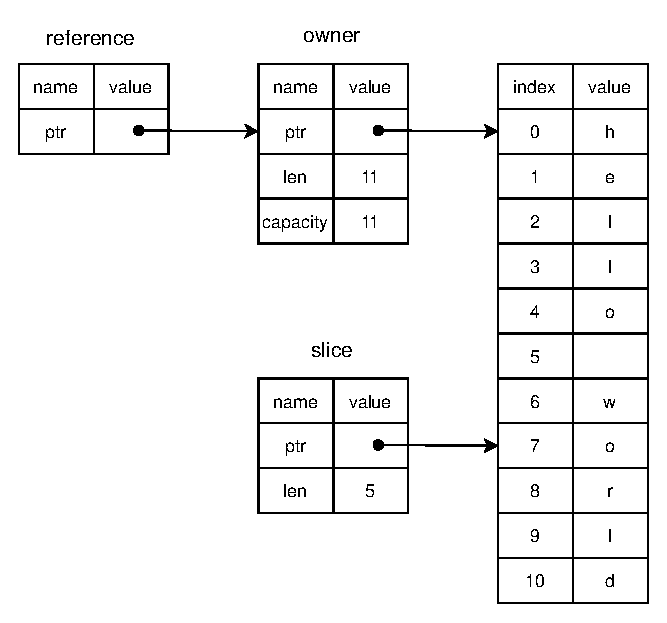
\includegraphics[width=0.5\textwidth]{images/own_ref_slice.eps}
                \captionsetup{labelformat=empty}
                % \caption{\textbf{}}
        \end{center}
    \end{figure}

    Each one may have \textcolor{blue}{different memory access time.}
\end{frame}

%%%%%%%%%%%%%%%%%%%%%%%%%%%%%%%%%%%%%%%%%%%%
%%%%%%%%%%%%%%%%%%%%%%%%%%%%%%%%%%%%%%%%%%%%

\begin{frame}[fragile]{Reference Counting}

    \textbf{Advantage}
    \begin{itemize}
        \item \blue{Sharing ownership} 
        \item \blue{Dinamic memory de/allocation}
    \end{itemize}

    \vspace{0.5cm}

    \textbf{Disadvantage}
    \begin{itemize}
        \item \blue{Need to check reference count} 
        \item \blue{Heap allocation}
    \end{itemize}


\end{frame}


%%%%%%%%%%%%%%%%%%%%%%%%%%%%%%%%%%%%%%%%%%%%
%%%%%%%%%%%%%%%%%%%%%%%%%%%%%%%%%%%%%%%%%%%%

\begin{frame}[fragile]{Complex Object - Memory Ownership and Borrowing}

A Complex Object like a nested Customer Object like those defined in the complete Web-based shop. 
 

\centering
\begin{minipage}{0.8\linewidth}
\begin{lstlisting}[title={Memory Ownership},language=Rust]
struct CustomerOwned {
		key: i32,
		total_purchase: f64,
		zip_code: String,
		order: OrderOwned
		... 10 more 
        }
\end{lstlisting}
\end{minipage}    


\begin{minipage}{0.8\linewidth}
\begin{lstlisting}[title={Memory Borrowing},language=Rust]

struct CustomerBorrowed<'a> {
		key: &'a i32,
		total_purchase: &'a f64,
		zip_code: &'a String,
		order: &'a OrderBorrowed<'a>
		... 10 more 
        }
\end{lstlisting}
\end{minipage}    
\end{frame}




%%%%%%%%%%%%%%%%%%%%%%%%%%%%%%%%%%%%%%%%%%%%
%%%%%%%%%%%%%%%%%%%%%%%%%%%%%%%%%%%%%%%%%%%%

\begin{frame}[t,fragile]{Complex Object - Slicing and Reference Counting }

%Memory Slicing and Atomic Reference Counting 
CustomerSlice has slices of String instead of reference of String
\centering
    
\begin{minipage}{0.8\linewidth}
\begin{lstlisting}[title={Memory Slicing},language=Rust]

struct CustomerSlice<'a> {
		key: &'a i32,
		total_purchase: &'a f64,
		zip_code: &'a str,
		order: &'a OrderSlice<'a>
        		... 10 more 
         }
\end{lstlisting}
\end{minipage}    

\begin{minipage}{0.8\linewidth}
\begin{lstlisting}[title={Atomic Reference Counting },language=Rust]

struct CustomerRc {
		key: Rc<i32>,
		total_purchase: Rc<f64>,
		zip_code: Rc<String>,
		order: Rc<OrderRc>
		      		... 10 more 
        }
\end{lstlisting}
\end{minipage}   

\end{frame}

%%%%%%%%%%%%%%%%%%%%%%%%%%%%%%%%%%%%%%%%%%%%
%%%%%%%%%%%%%%%%%%%%%%%%%%%%%%%%%%%%%%%%%%%%

\begin{frame}[fragile]{Multithreading with Atomic Reference Counting}
    Atomic Reference Counting

    \vspace{0.5cm}
    \textbf{Advantage}
    \begin{itemize}
        \item \blue{Sharing ownership} 
        \item \blue{Dinamic memory de/allocation}
        \item \blue{Sharing among multithreads}
    \end{itemize}

    \vspace{0.5cm}

    \textbf{Disadvantage}
    \begin{itemize}
        \item \blue{Need to check reference count} 
        \item \blue{Heap allocation}
        \item \blue{Atomic operation} 
    \end{itemize}

\end{frame}

%%%%%%%%%%%%%%%%%%%%%%%%%%%%%%%%%%%%%%%%%%%%
%%%%%%%%%%%%%%%%%%%%%%%%%%%%%%%%%%%%%%%%%%%%

\begin{frame}[fragile]{Impact of Memory Management on performance of Big Data Processing}

    \begin{itemize}
        \item \blueb{Merge-sort}
        \begin{itemize}
            \item Many contiguous memory de/allocations
        \end{itemize}
        \vspace{0.5cm}
        \item \blueb{Tree-aggtegate}
        \begin{itemize}
            \item Many intermediate HashMap like data structures
        \end{itemize}
        \vspace{0.5cm}
        \item \blueb{K-Nearest-Neighbors (KNN)}
        \begin{itemize}
            \item Document preprocessing 
        \end{itemize}    
    \end{itemize}

\end{frame}

%%%%%%%%%%%%%%%%%%%%%%%%%%%%%%%%%%%%%%%%%%%%
%%%%%%%%%%%%%%%%%%%%%%%%%%%%%%%%%%%%%%%%%%%%

\begin{frame}[fragile]{Experiment 1: Accessing Object with Different Variable Type}

    \textbf{Question}
    \begin{itemize}
        \item How much memory access time are different among different memory management strategies used in complex objects specification?
    \end{itemize}

    \vspace{0.5cm}

    \textbf{Evaluation}
    \begin{itemize}
        \item \blueb{Construct Complex objects}
        \item With different memory management strategies: \blueb{Owner, Reference, Slice}
        \item \textbf{CustomerOwned} vs. \textbf{CustomerBorrowed} vs. \textbf{CustomerSlice}
        \item Measure access time of different \blueb{fields of complex objects}
    \end{itemize}

\end{frame}

%%%%%%%%%%%%%%%%%%%%%%%%%%%%%%%%%%%%%%%%%%%%
%%%%%%%%%%%%%%%%%%%%%%%%%%%%%%%%%%%%%%%%%%%%

\begin{frame}[t, fragile]{Experiment 1: Accessing Object with Different Variable Type}

    \begin{figure}[hp]
        \centering
        \begin{center}
                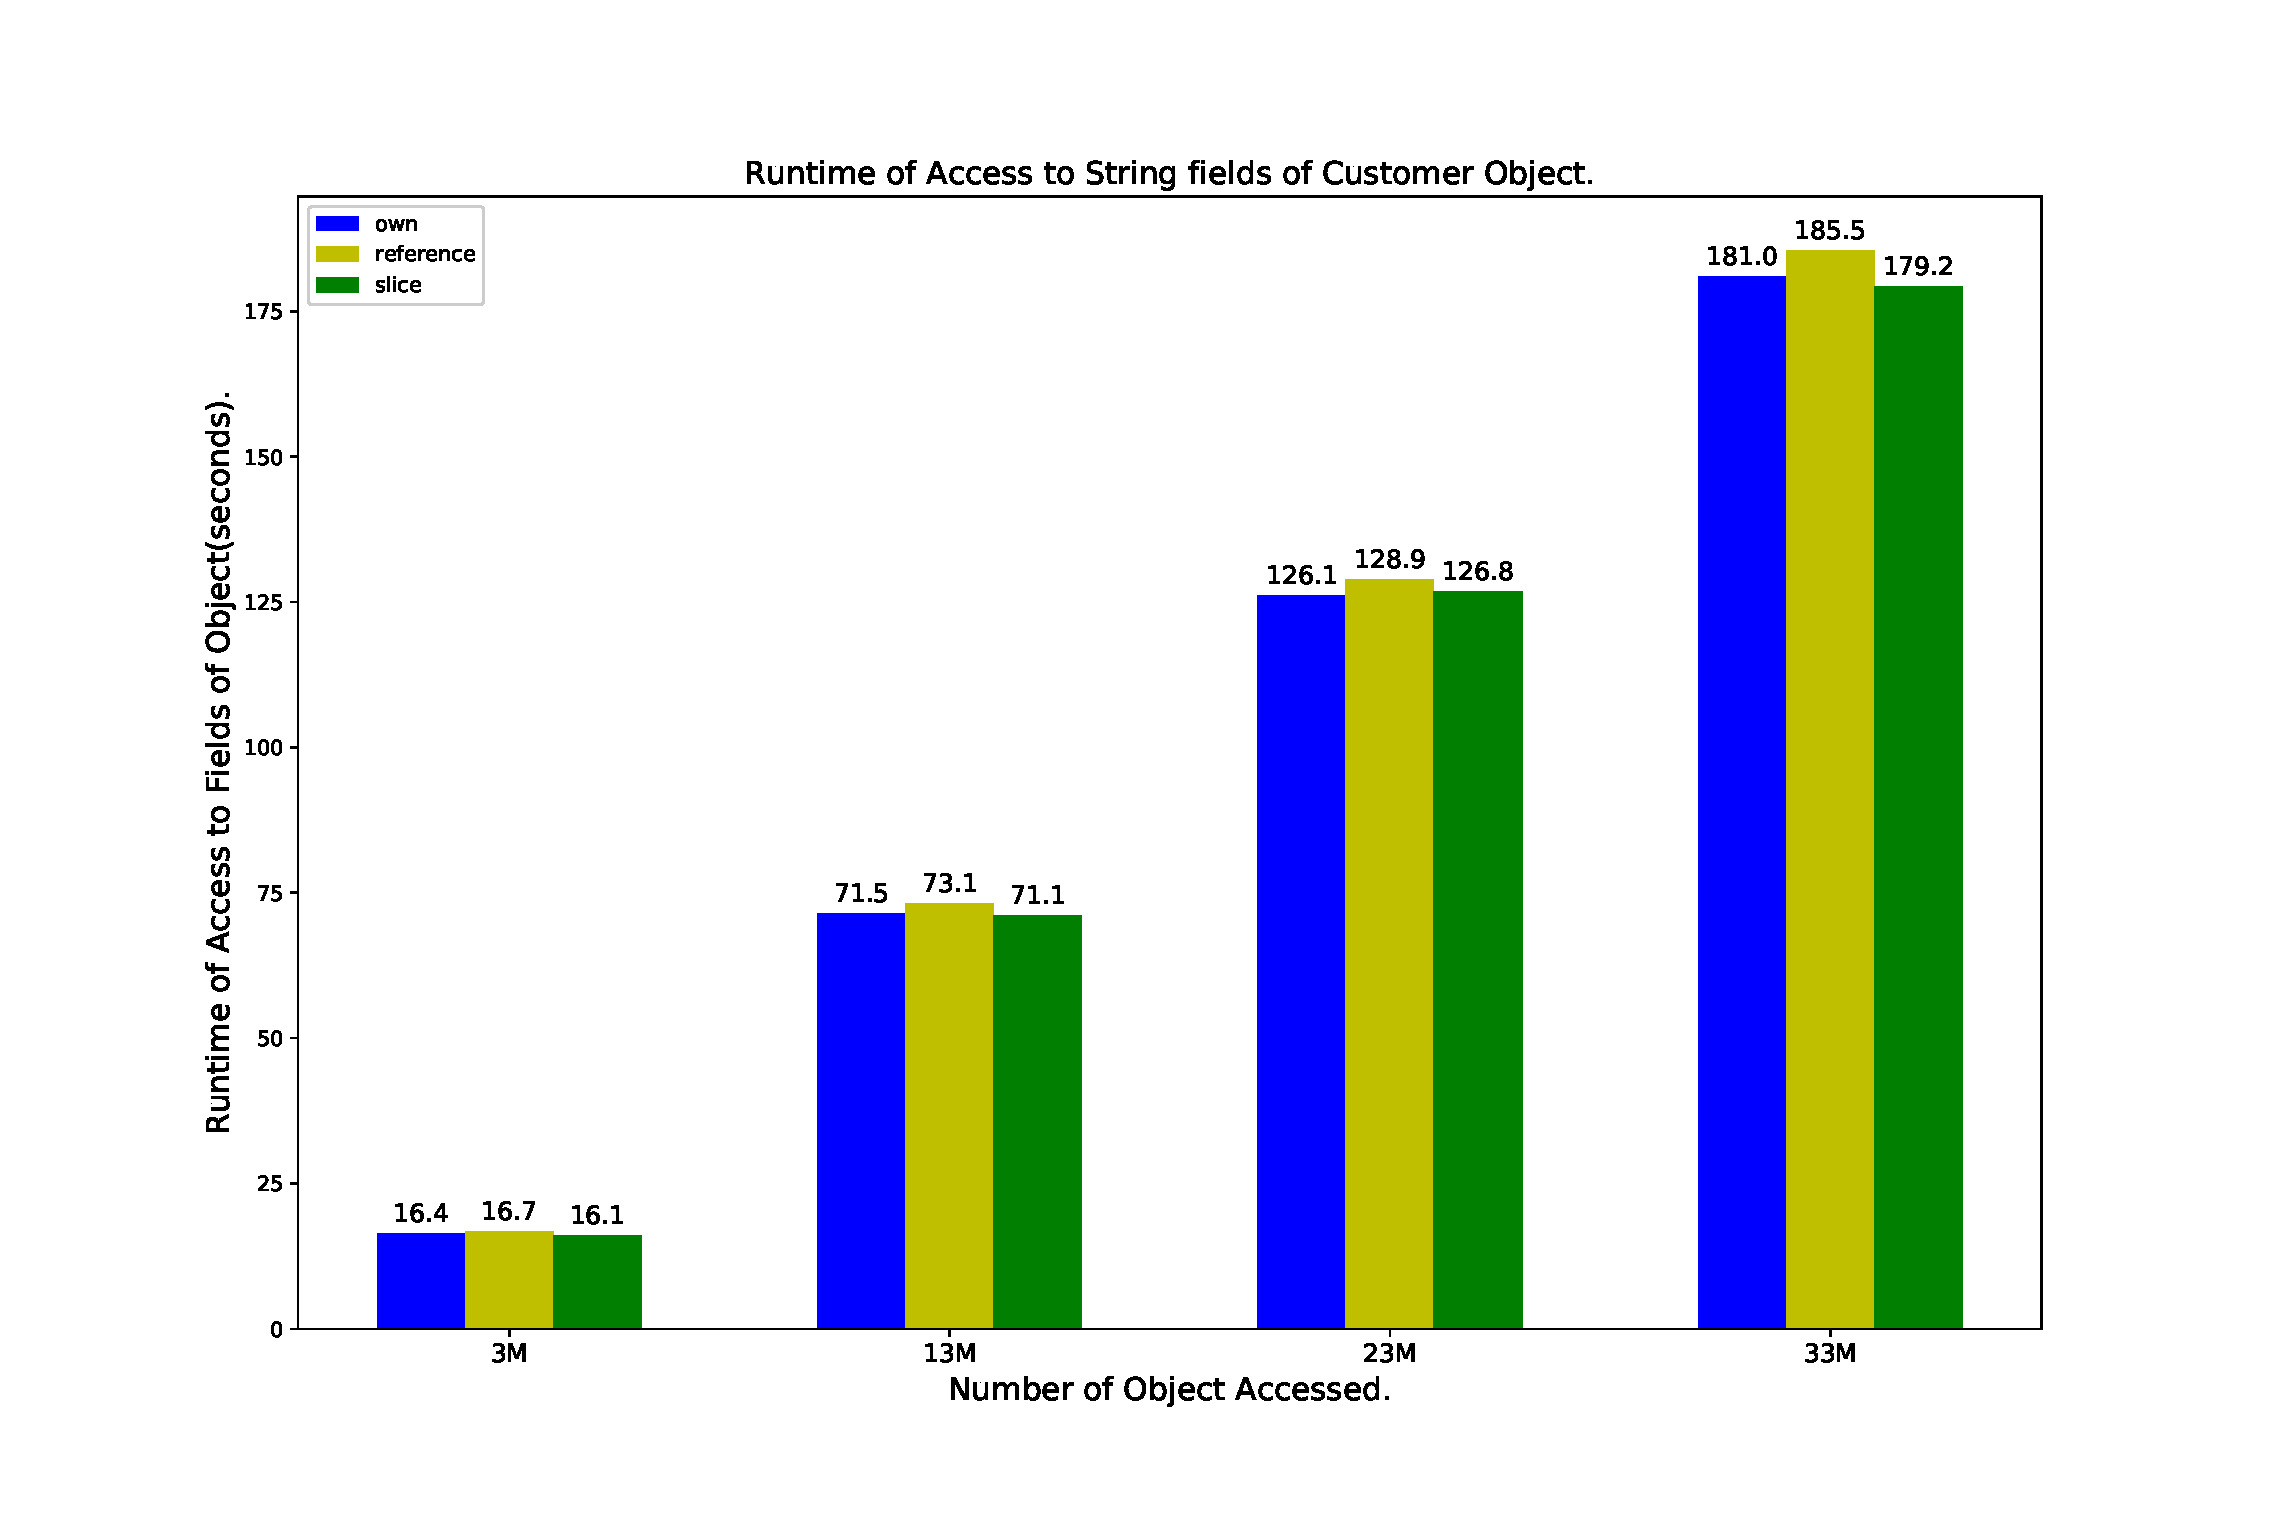
\includegraphics[width=1\textwidth]{images/rust_access_different_poniter_init.eps}
                \captionsetup{labelformat=empty}
                % \caption{\textbf{}}
        \end{center}
    \end{figure}
\end{frame}

%%%%%%%%%%%%%%%%%%%%%%%%%%%%%%%%%%%%%%%%%%%%
%%%%%%%%%%%%%%%%%%%%%%%%%%%%%%%%%%%%%%%%%%%%

\begin{frame}[fragile]{Experiment 2: Assessment of different reference methods in Rust}

    \textbf{Question}
    \begin{itemize}
        \item How much does Reference Counting hits performance?
    \end{itemize}

    \vspace{0.5cm}

    \textbf{Evaluation}
    \begin{itemize}
        \item \blueb{Custruct complext objects}
        \item \blueb{Reference Counting} vs \blueb{reference}
        \item CustomerRc vs. CustomerBorrowed
        \item Measure time to \blueb{drop variables of complex objects}
    \end{itemize}

\end{frame}

%%%%%%%%%%%%%%%%%%%%%%%%%%%%%%%%%%%%%%%%%%%%
%%%%%%%%%%%%%%%%%%%%%%%%%%%%%%%%%%%%%%%%%%%%


\begin{frame}[fragile]{Experiment 2: Assessment of different reference methods in Rust}

    \begin{figure}[hp]
        \centering
        \begin{center}
                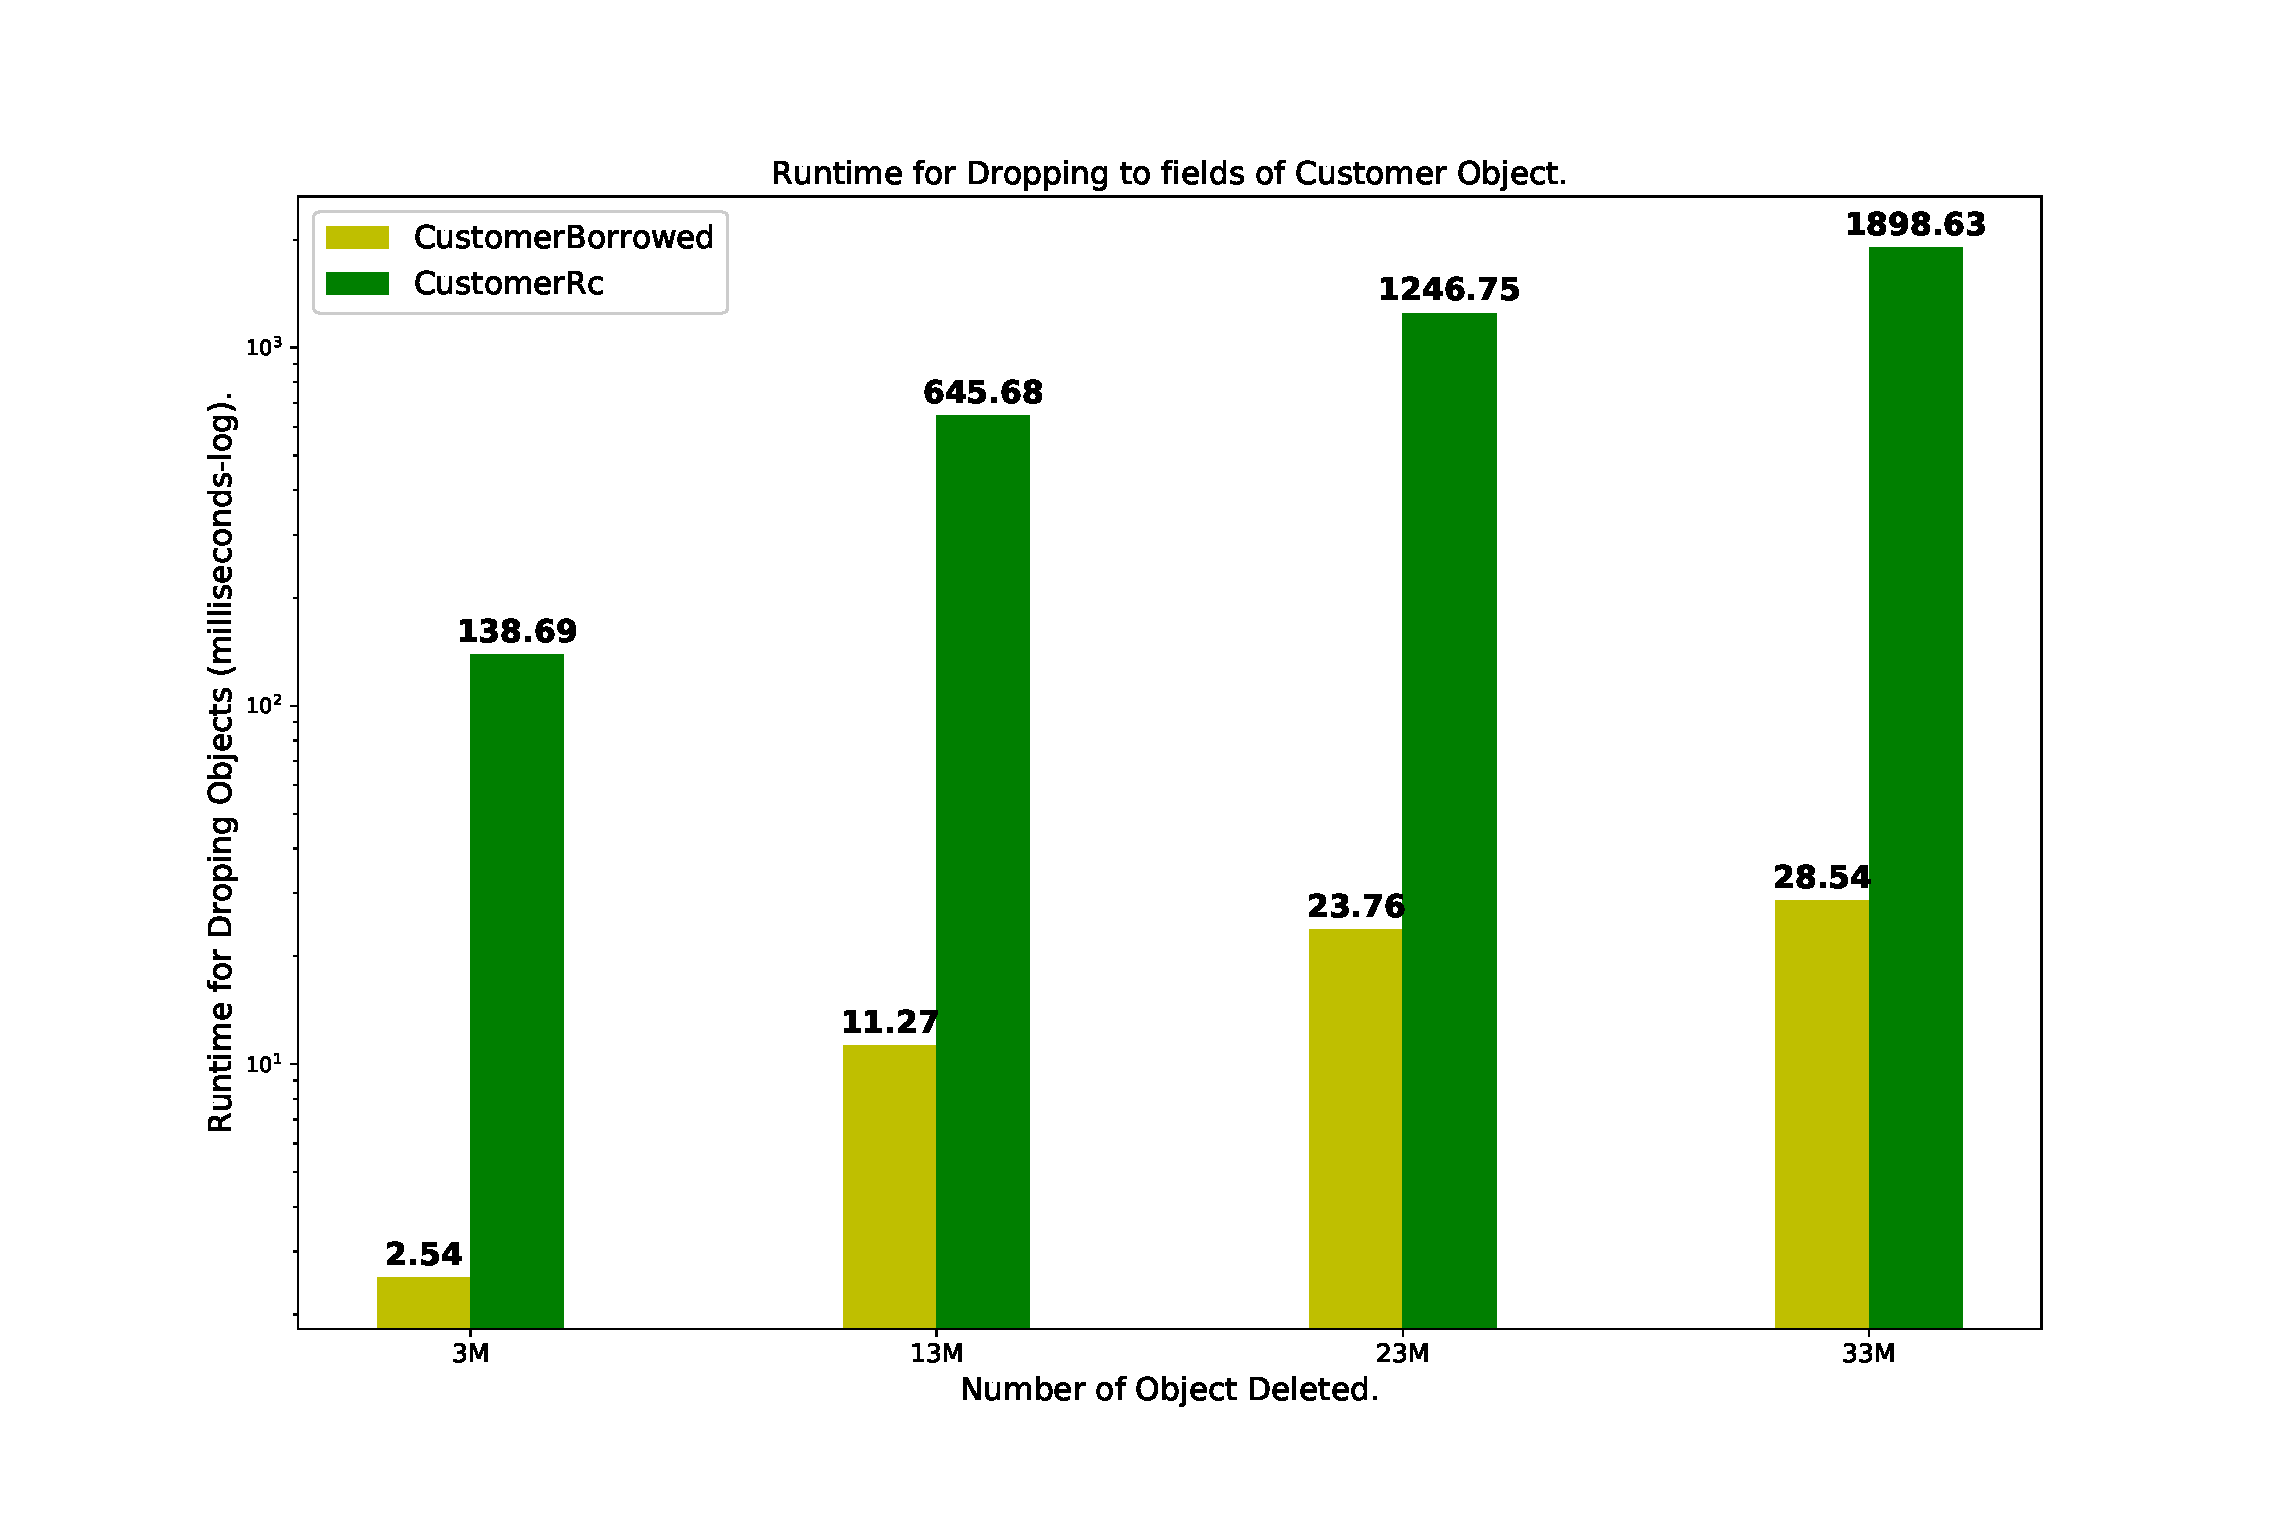
\includegraphics[width=1\textwidth]{images/rust_droptime_borring_rc.eps}
                \captionsetup{labelformat=empty}
                % \caption{\textbf{}}
        \end{center}
    \end{figure}
\end{frame}
%%%%%%%%%%%%%%%%%%%%%%%%%%%%%%%%%%%%%%%%%%%%
%%%%%%%%%%%%%%%%%%%%%%%%%%%%%%%%%%%%%%%%%%%%

\begin{frame}[fragile]{Experiment 2: Assessment of different reference methods in Rust}
    \textbf{Result}
    \begin{itemize}
        \item Dropping Reference Counting is about \blueb{60 times slower} than normal reference.
    \end{itemize}

    \vspace{0.5cm}

    \textbf{Discussion}
    \begin{itemize}
        \item Reference Counting needs some CPU cycles to check reference count.
        \item In complex objects, overhead is significant.
    \end{itemize}
\end{frame}

%%%%%%%%%%%%%%%%%%%%%%%%%%%%%%%%%%%%%%%%%%%%
%%%%%%%%%%%%%%%%%%%%%%%%%%%%%%%%%%%%%%%%%%%%

\begin{frame}[fragile]{Experiment 3: Merge-sort}

    \textbf{Question}
    \begin{itemize}
        \item How much does sharing set of data with Atomic Reference Counting have impact on performance of merge-sort algorithms?
    \end{itemize}

    \vspace{0.5cm}

    \textbf{Evaluation}
    \begin{itemize}
        \item Share \blueb{vector} of complex objects
        \item \blueb{Atomic Reference Counting (Arc)} vs \blueb{normal reference}
        \item Measure \blueb{runtime of merge-sort algorithms}
    \end{itemize}
\end{frame}

%%%%%%%%%%%%%%%%%%%%%%%%%%%%%%%%%%%%%%%%%%%%
%%%%%%%%%%%%%%%%%%%%%%%%%%%%%%%%%%%%%%%%%%%%


\begin{frame}[fragile]{Experiment 3: Merge-sort}
    \vspace{-0.7cm}
    \begin{figure}[hp]
        \centering
        \begin{center}
                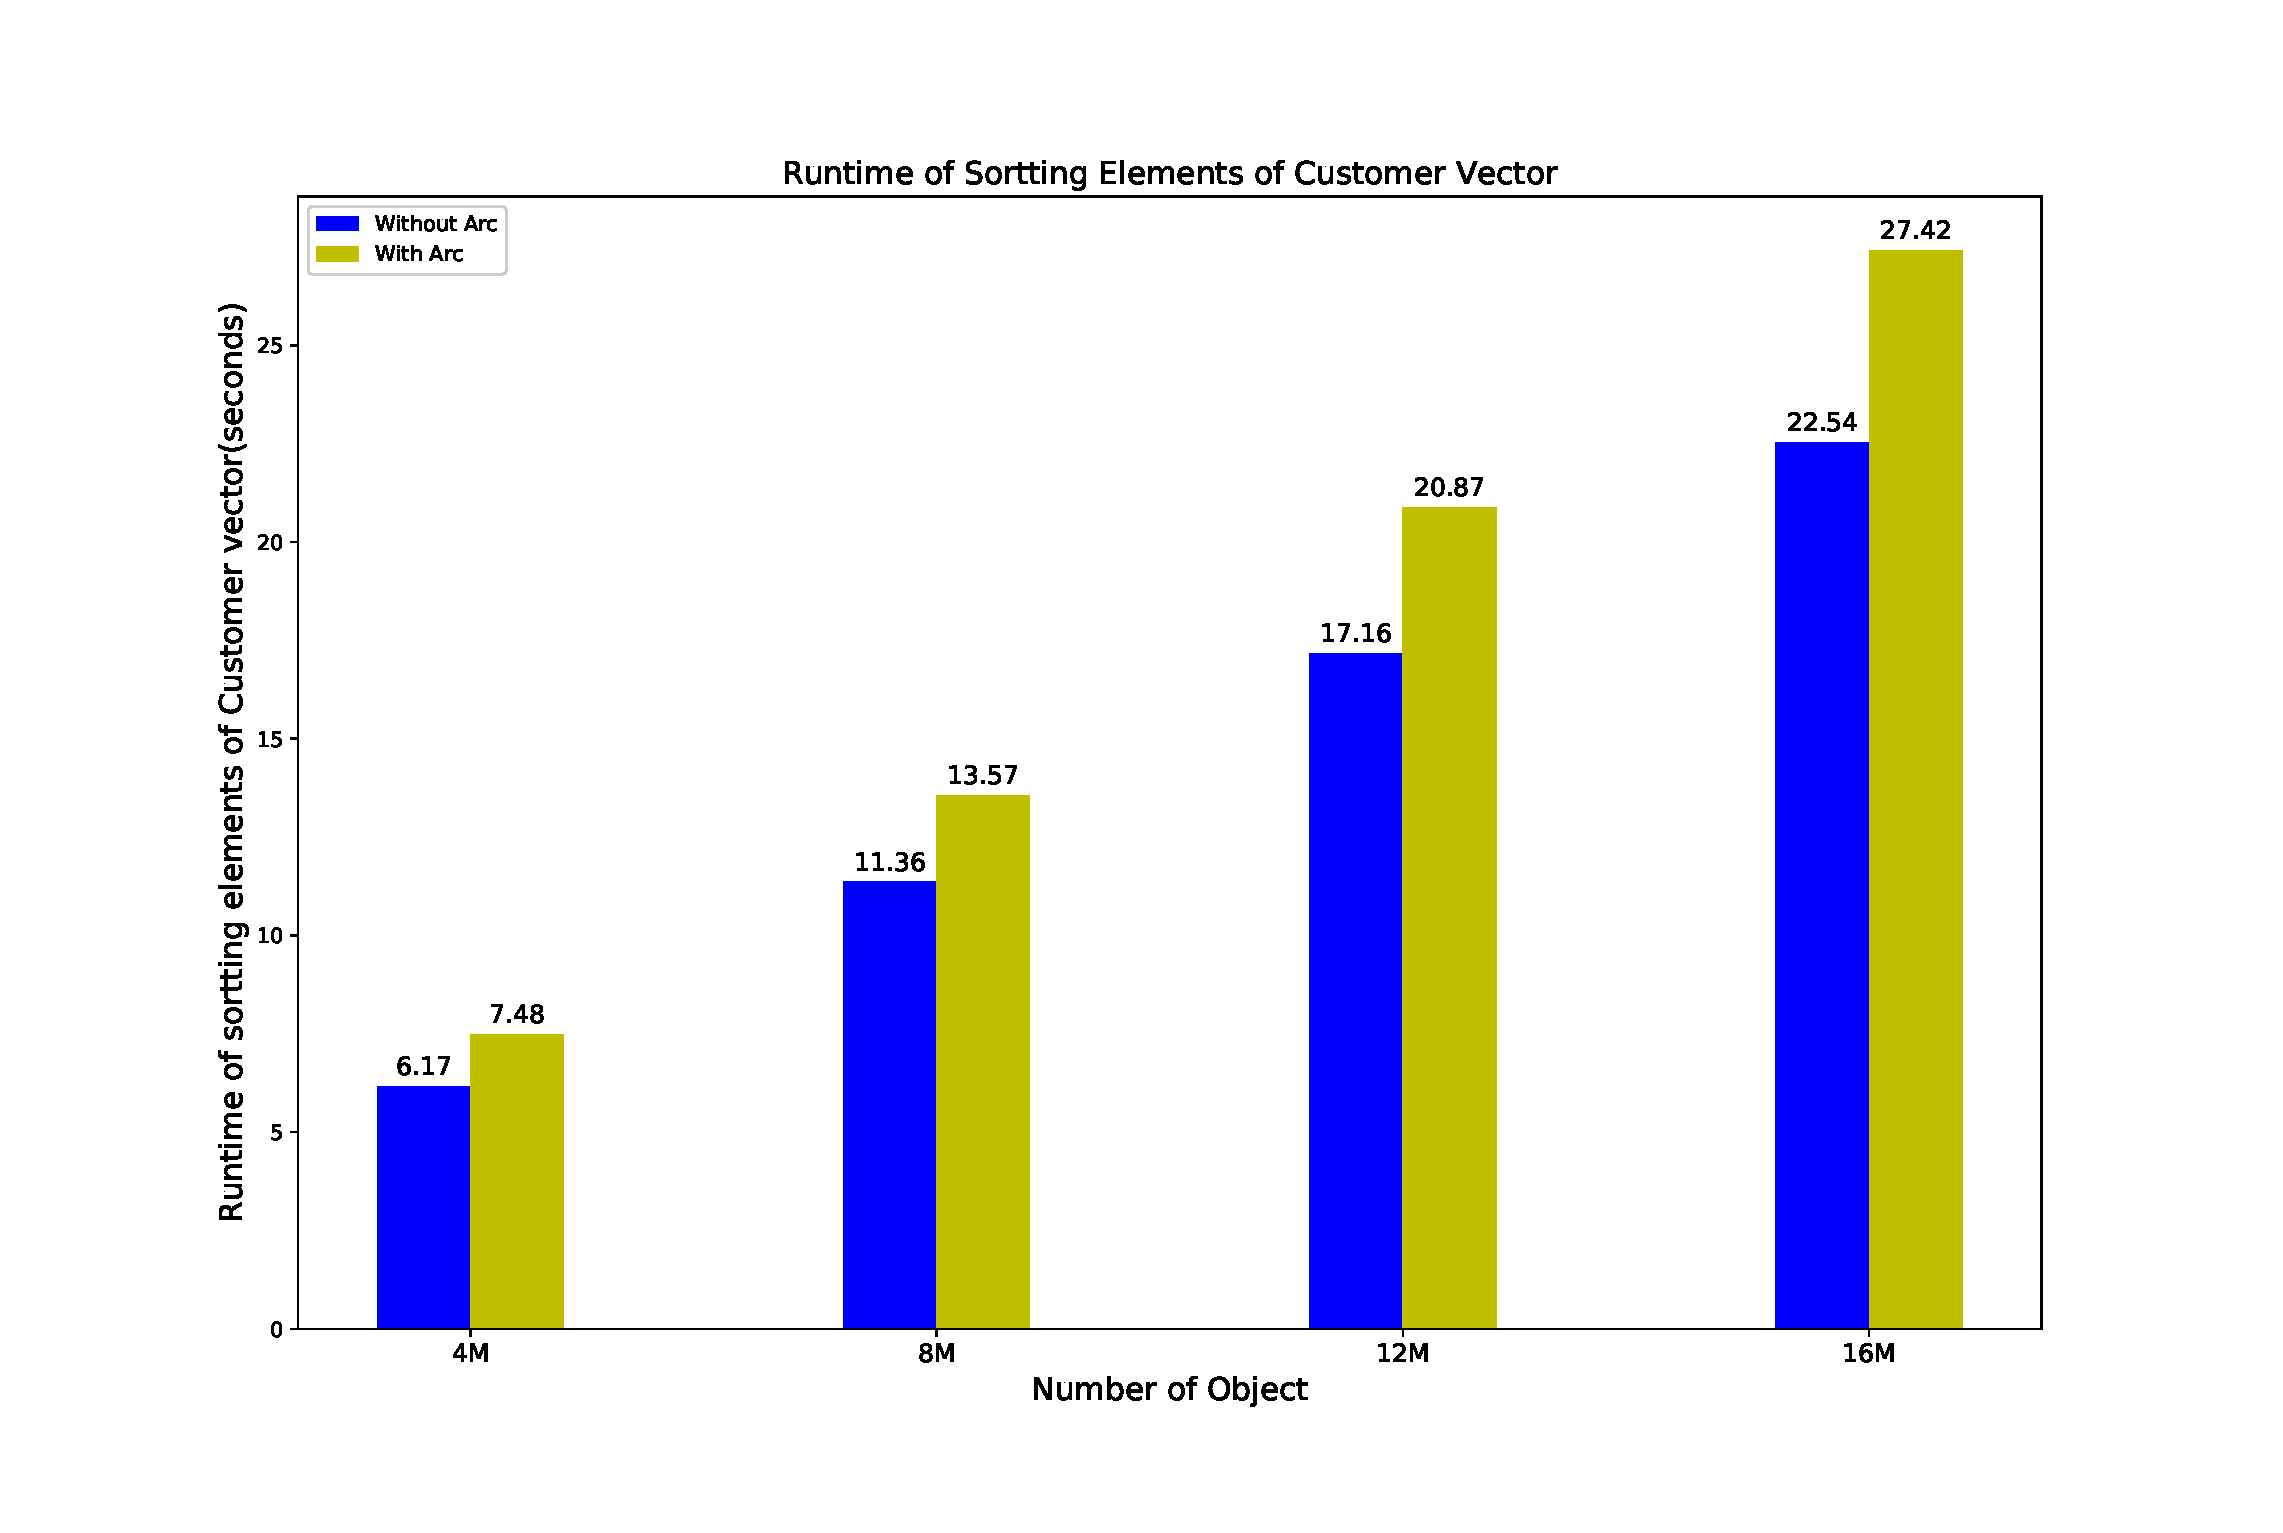
\includegraphics[width=1.1\textwidth]{images/rust_merge_sort.eps}
                \captionsetup{labelformat=empty}
                % \caption{\textbf{}}
        \end{center}
    \end{figure}
\end{frame}

%%%%%%%%%%%%%%%%%%%%%%%%%%%%%%%%%%%%%%%%%%%%
%%%%%%%%%%%%%%%%%%%%%%%%%%%%%%%%%%%%%%%%%%%%

\begin{frame}[fragile]{Experiment 3: Merge-sort}

    \textbf{Result}
    \begin{itemize}
        \item Arc are about \blueb{21\%  slower} than normal reference.
    \end{itemize}

    \vspace{0.5cm}

    \textbf{Discussion}
    \begin{itemize}
        \item Atomic Reference Counting needs to check reference count.
        \item Atomic operations are more expensive than ordinal operations.
    \end{itemize}

\end{frame}

%%%%%%%%%%%%%%%%%%%%%%%%%%%%%%%%%%%%%%%%%%%%
%%%%%%%%%%%%%%%%%%%%%%%%%%%%%%%%%%%%%%%%%%%%

\begin{frame}[fragile]{Experiment 4: Tree-aggregate}

    \textbf{Question}
    \begin{itemize}
        \item How much are runtime differences between sharing elements of data with Arc and deep-copying elements of data?
    \end{itemize}

    \vspace{0.5cm}

    \textbf{Evaluation}
    \begin{itemize}
        \item Share \blueb{elements} of complex object
        \item \blueb{Atomic Reference Counting (ARC)} vs \blueb{Deep copy}
        \item Measure \blueb{runtime of Tree-aggregate algorithms}
    \end{itemize}

\end{frame}

%%%%%%%%%%%%%%%%%%%%%%%%%%%%%%%%%%%%%%%%%%%%
%%%%%%%%%%%%%%%%%%%%%%%%%%%%%%%%%%%%%%%%%%%%

\begin{frame}[t, fragile]{Experiment 4: Tree-aggregate}
    \vspace{-0.7cm}
    \begin{figure}[hp]
        \centering
        \begin{center}
                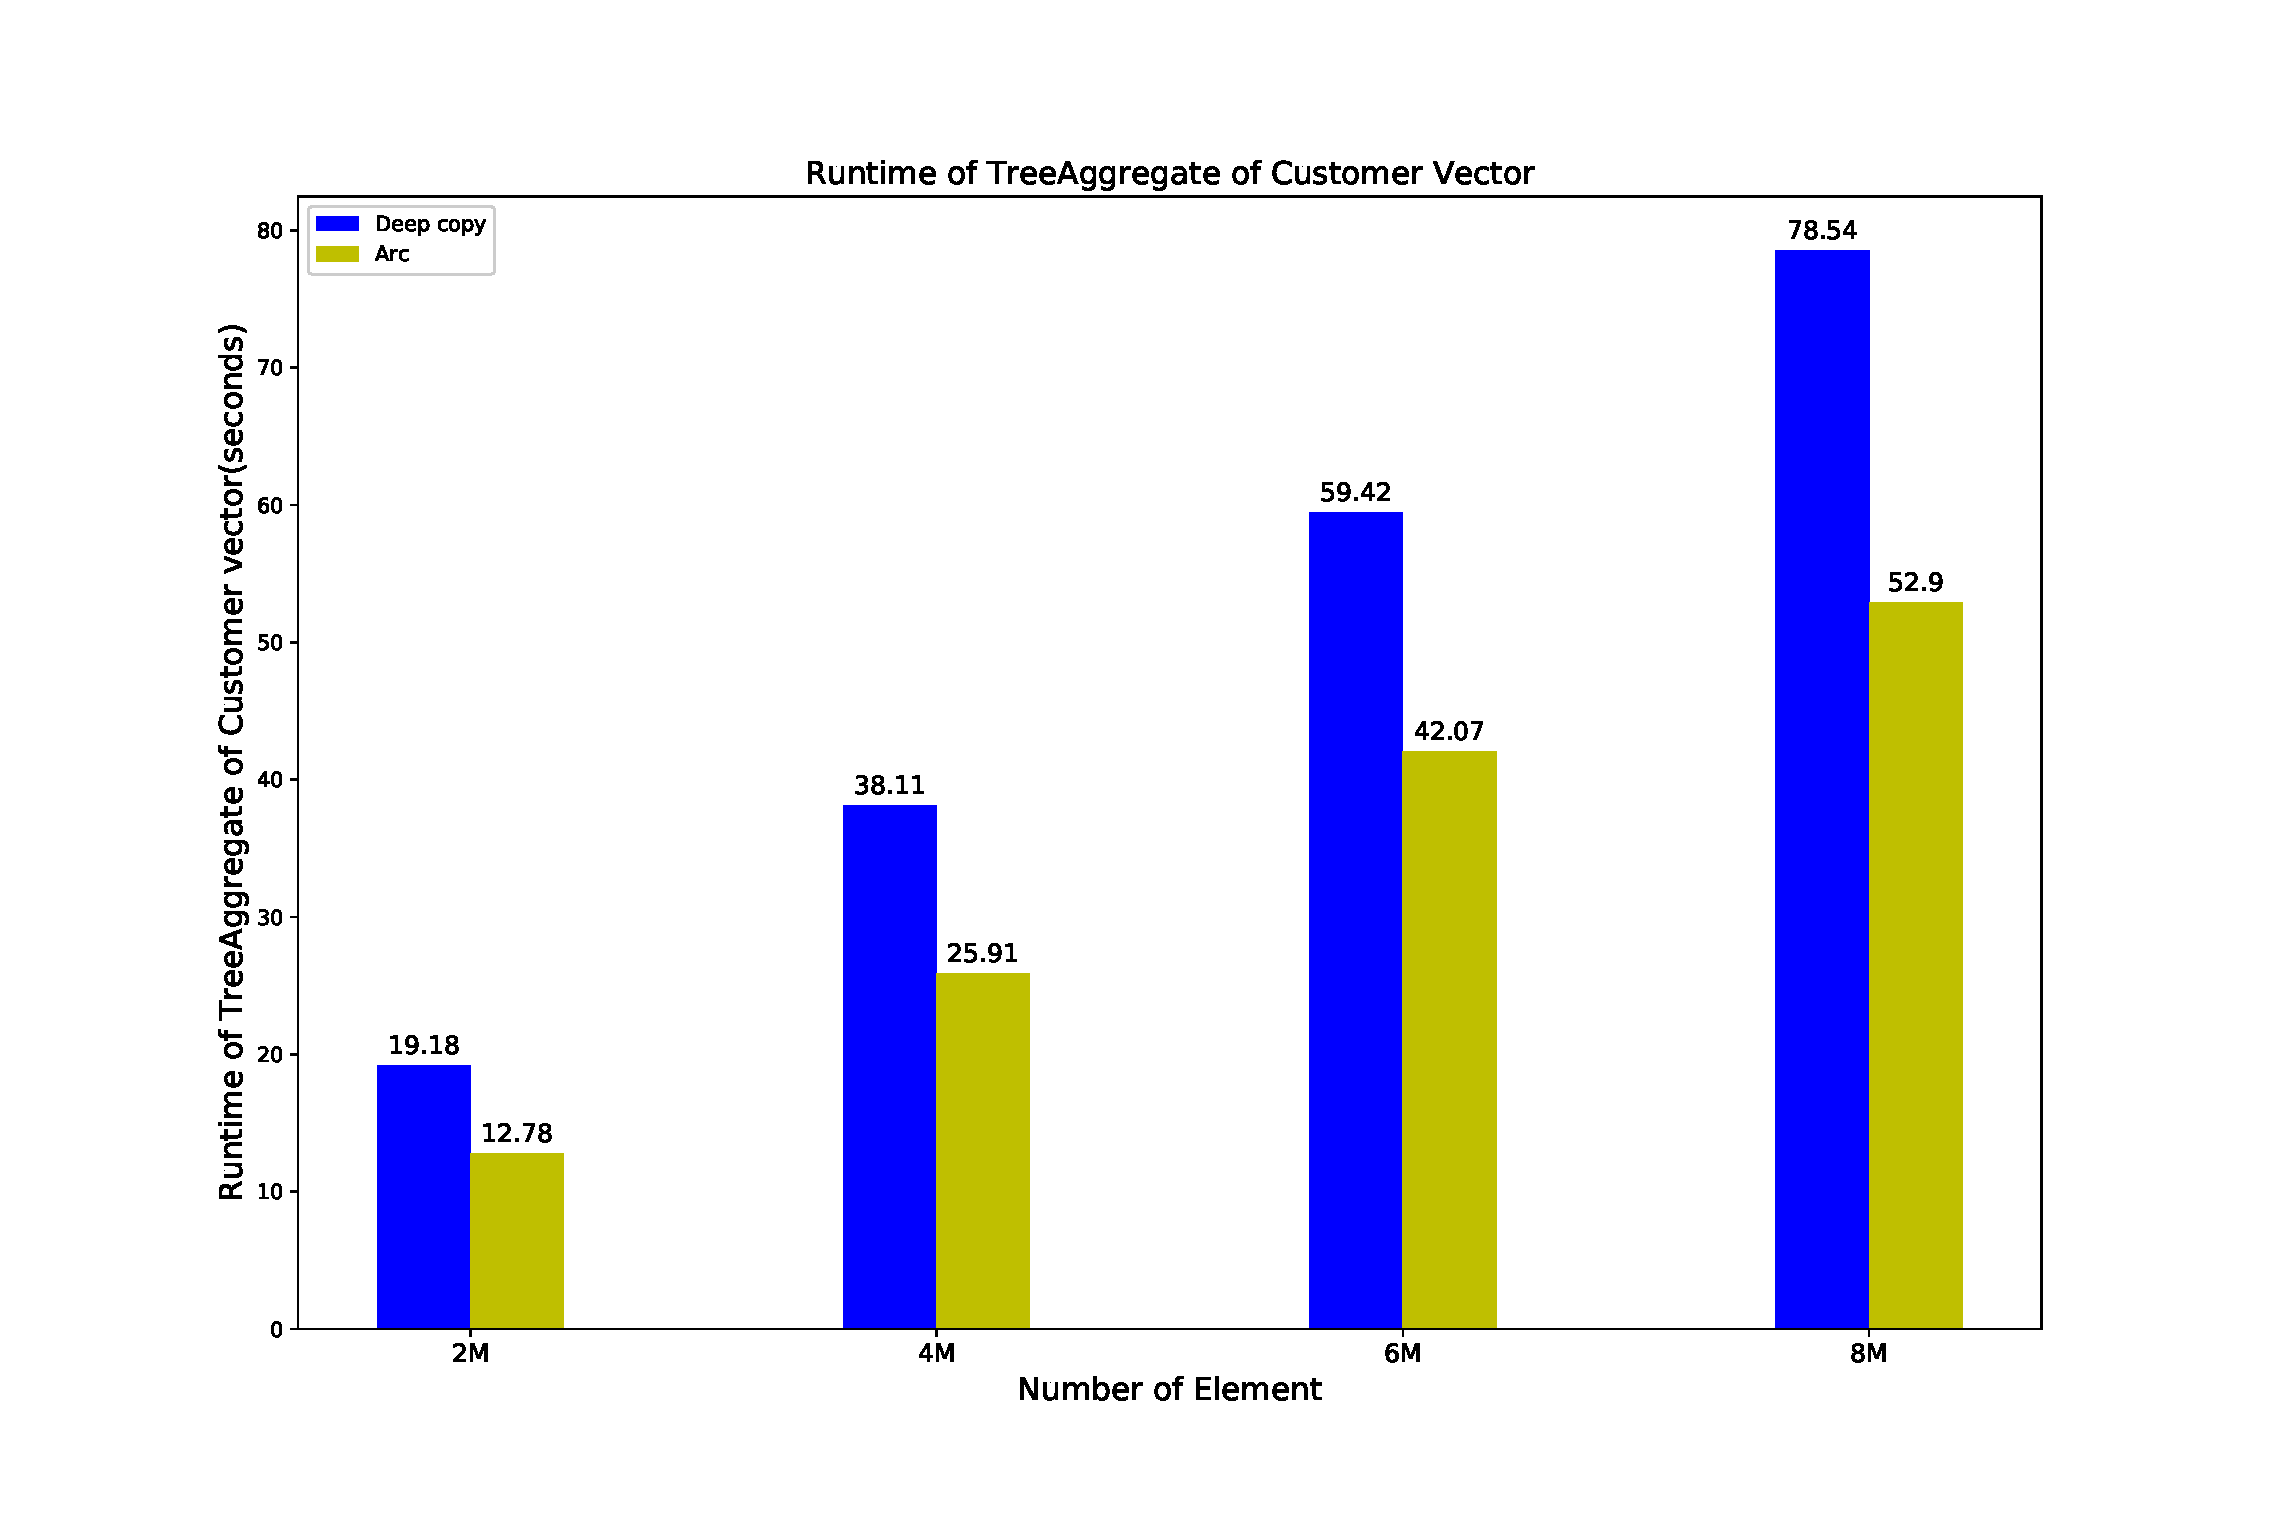
\includegraphics[width=1.1\textwidth]{images/rust_tree_aggregate.eps}
                \captionsetup{labelformat=empty}
                % \caption{\textbf{}}
        \end{center}
    \end{figure}
\end{frame}

%%%%%%%%%%%%%%%%%%%%%%%%%%%%%%%%%%%%%%%%%%%%
%%%%%%%%%%%%%%%%%%%%%%%%%%%%%%%%%%%%%%%%%%%%

\begin{frame}[fragile]{Experiment 4: Tree-aggregate}

    \textbf{Result}
    \begin{itemize}
        \item Deep-copies are from \blueb{40 to 50\% slower} than Arc.
    \end{itemize}

    \vspace{0.5cm}

    \textbf{Discussion}
    \begin{itemize}
        \item Deep-copy of complex object is expensive.
        \item Performing deep-copy many times may lead significant overhead.
    \end{itemize}

\end{frame}

%%%%%%%%%%%%%%%%%%%%%%%%%%%%%%%%%%%%%%%%%%%%
%%%%%%%%%%%%%%%%%%%%%%%%%%%%%%%%%%%%%%%%%%%%
\begin{frame}[fragile]{Experiment 5: K-Nearest-Neighbors (KNN)}

    \textbf{Question}
    \begin{itemize}
        \item What are better memory management strategies for common Machine Learning Algorithms?
    \end{itemize}

    \vspace{0.5cm}

    \textbf{Evaluation}
    \begin{itemize}
        \item Document classification on Wikipedia page dataset
        \begin{itemize}
            \item train set: \(100 \times 10^3 \) pages
            \item test set: \(18 \times  10^3\) pages
        \end{itemize}
        \item Preprocessing phase: calculating \blueb{Term-Frequencies (TFs)}
        \item String manipulation
        \item Measure runtime of \blueb{preprocessing time of KNN algorithms}
    \end{itemize}
\end{frame}

%%%%%%%%%%%%%%%%%%%%%%%%%%%%%%%%%%%%%%%%%%%%
%%%%%%%%%%%%%%%%%%%%%%%%%%%%%%%%%%%%%%%%%%%%

\begin{frame}[fragile]{Experiment 5: K-Nearest-Neighbors (KNN)}

    \blueb{Parameters}
    \begin{itemize}
        \item Data Acquisition
        \begin{itemize}
            \item \blueb{Atomic Reference Counting} (Arc)
            \item \blueb{Deep-copy}
        \end{itemize} 
        \vspace{0.5cm}
        % \item Strategy
        % \begin{itemize}
        %     \item keep intermediate objects in memory until owner is changed
        %     \item remove intermediate objects as soon as it is not needed
        % \end{itemize}
        % \vspace{0.5cm}
        \item Dimensions of feature matrices
        \begin{itemize}
            \item 15K
            \item 20K
            \item 25K
        \end{itemize} 
    \end{itemize}
\end{frame}

%%%%%%%%%%%%%%%%%%%%%%%%%%%%%%%%%%%%%%%%%%%%
%%%%%%%%%%%%%%%%%%%%%%%%%%%%%%%%%%%%%%%%%%%%

\begin{frame}[fragile]{Experiment 5: K-Nearest-Neighbors}
    \vspace{-0.7cm}
    \begin{figure}[hp]
        \centering
        \begin{center}
                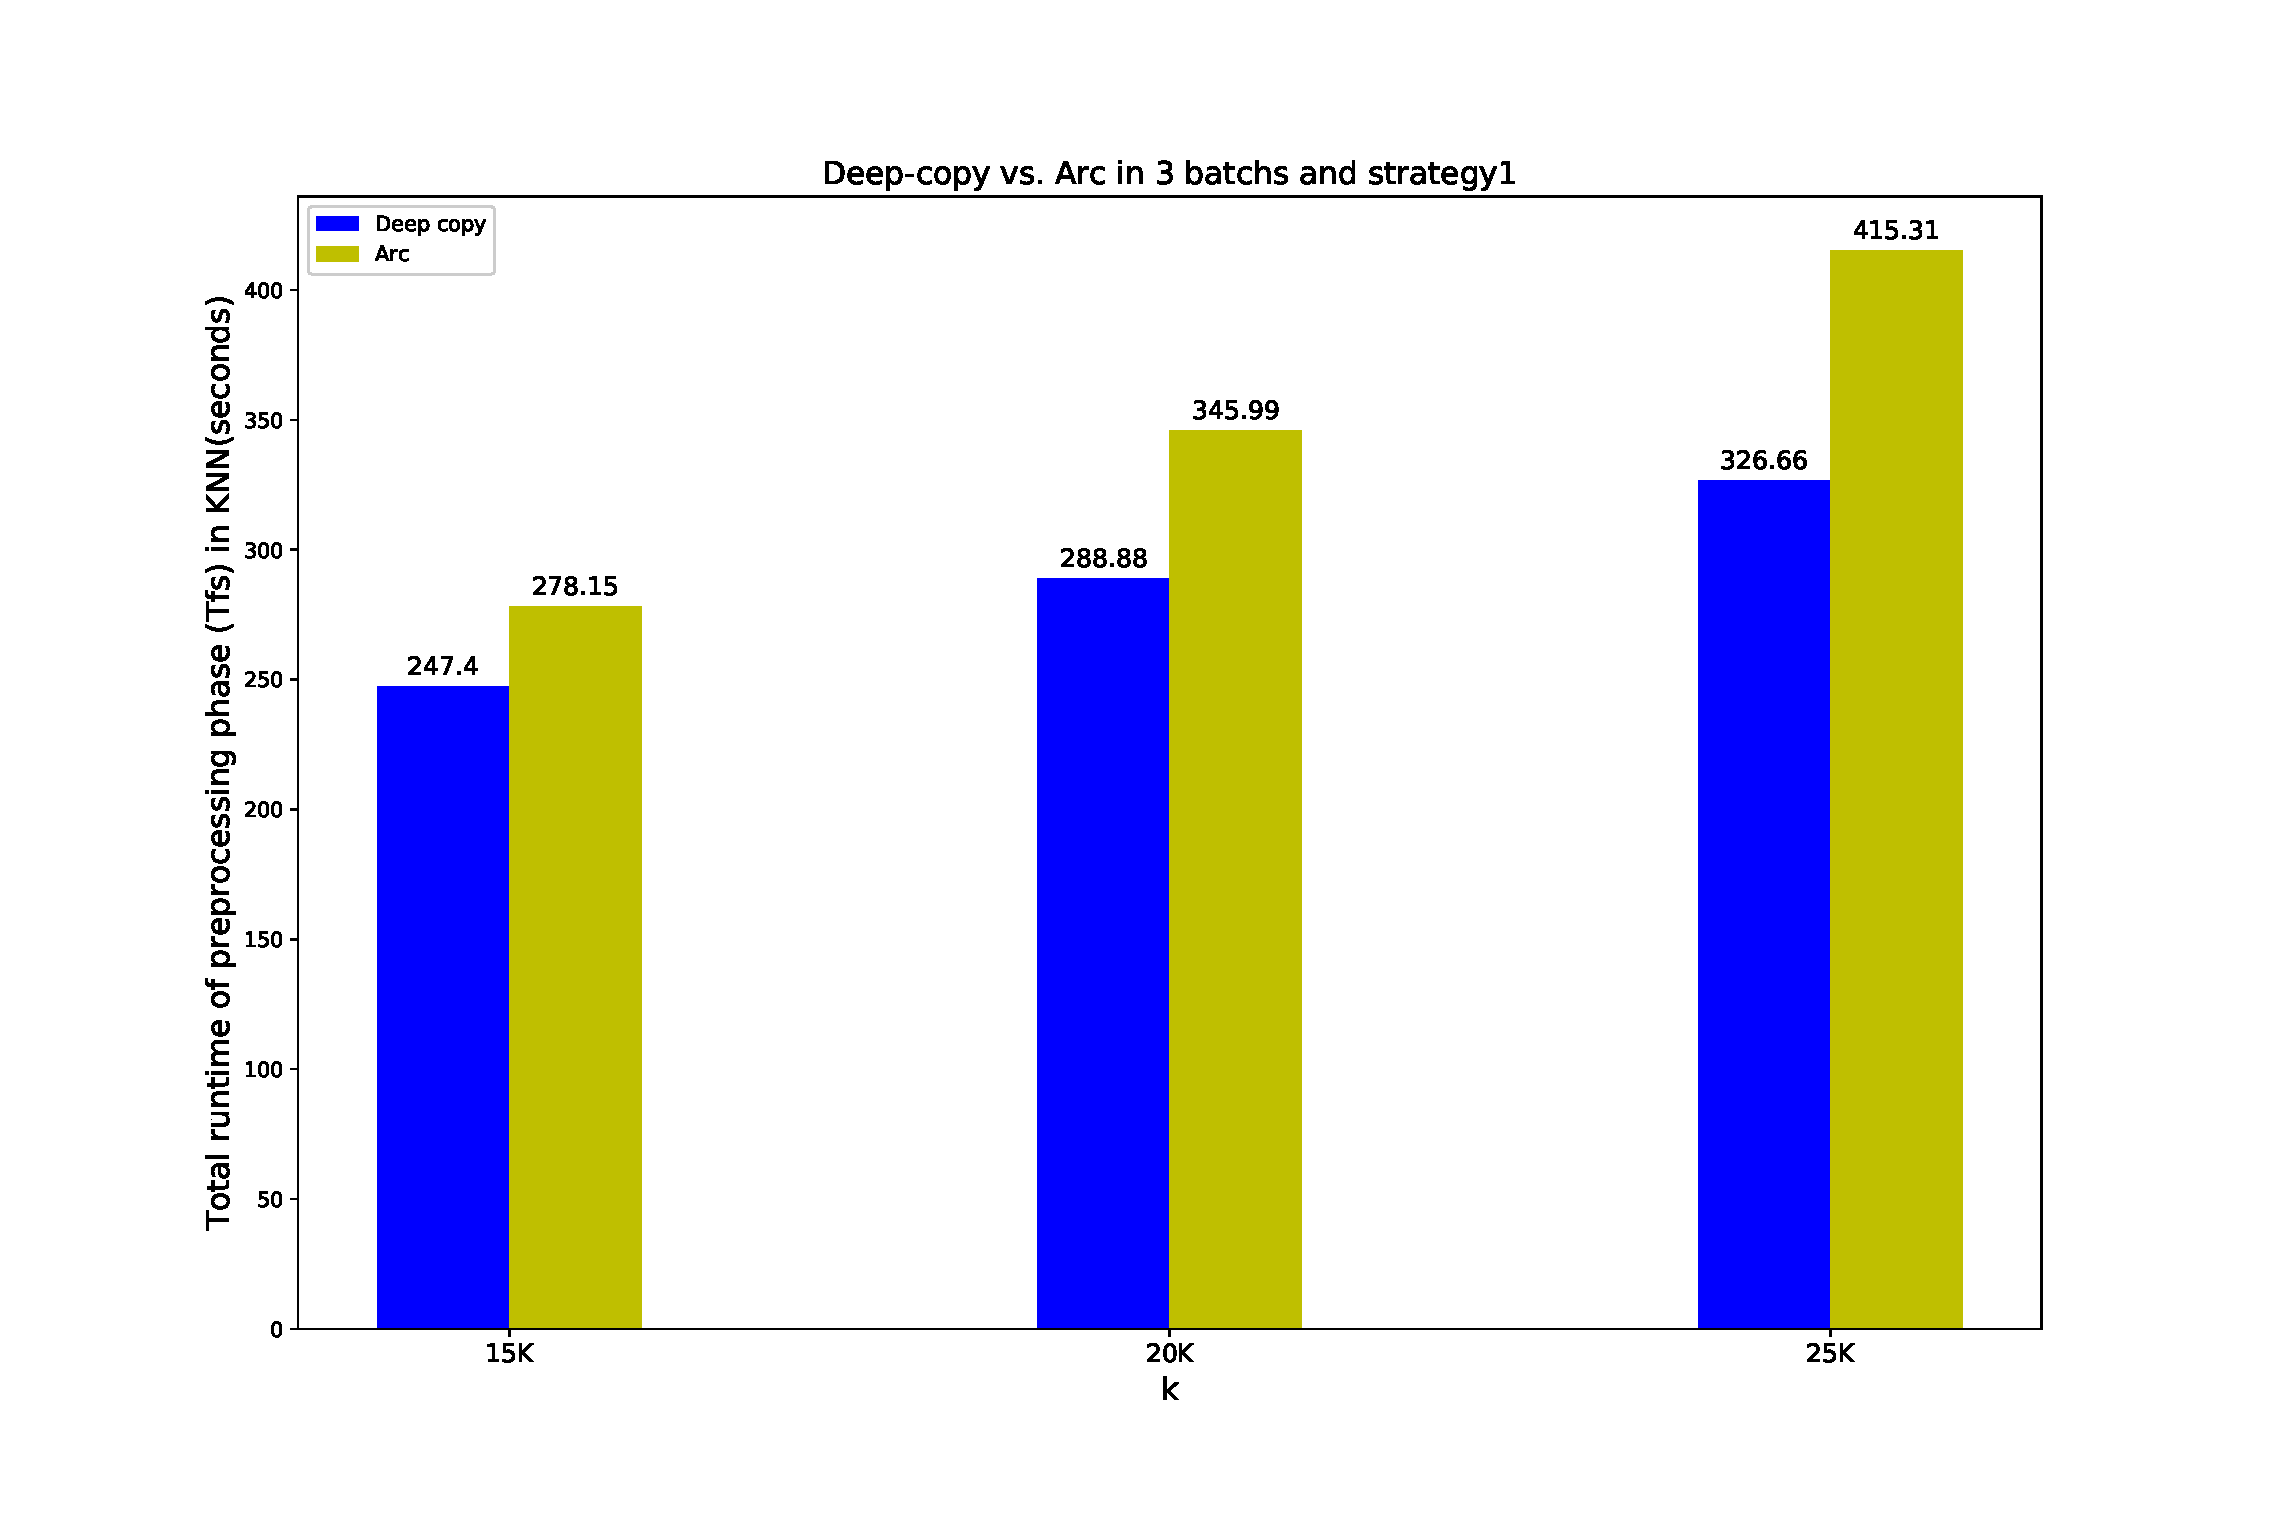
\includegraphics[width=1.1\textwidth]{images/deepcopy_vs_arc.eps}
                \captionsetup{labelformat=empty}
                % \caption{\textbf{}}
        \end{center}
    \end{figure}
    
\end{frame}

%%%%%%%%%%%%%%%%%%%%%%%%%%%%%%%%%%%%%%%%%%%%
%%%%%%%%%%%%%%%%%%%%%%%%%%%%%%%%%%%%%%%%%%%%

% \begin{frame}[fragile]{Experiment 5: K-Nearest-Neighbors}
%     \vspace{-0.7cm}
%     \begin{figure}[hp]
%         \centering
%         \begin{center}
%                 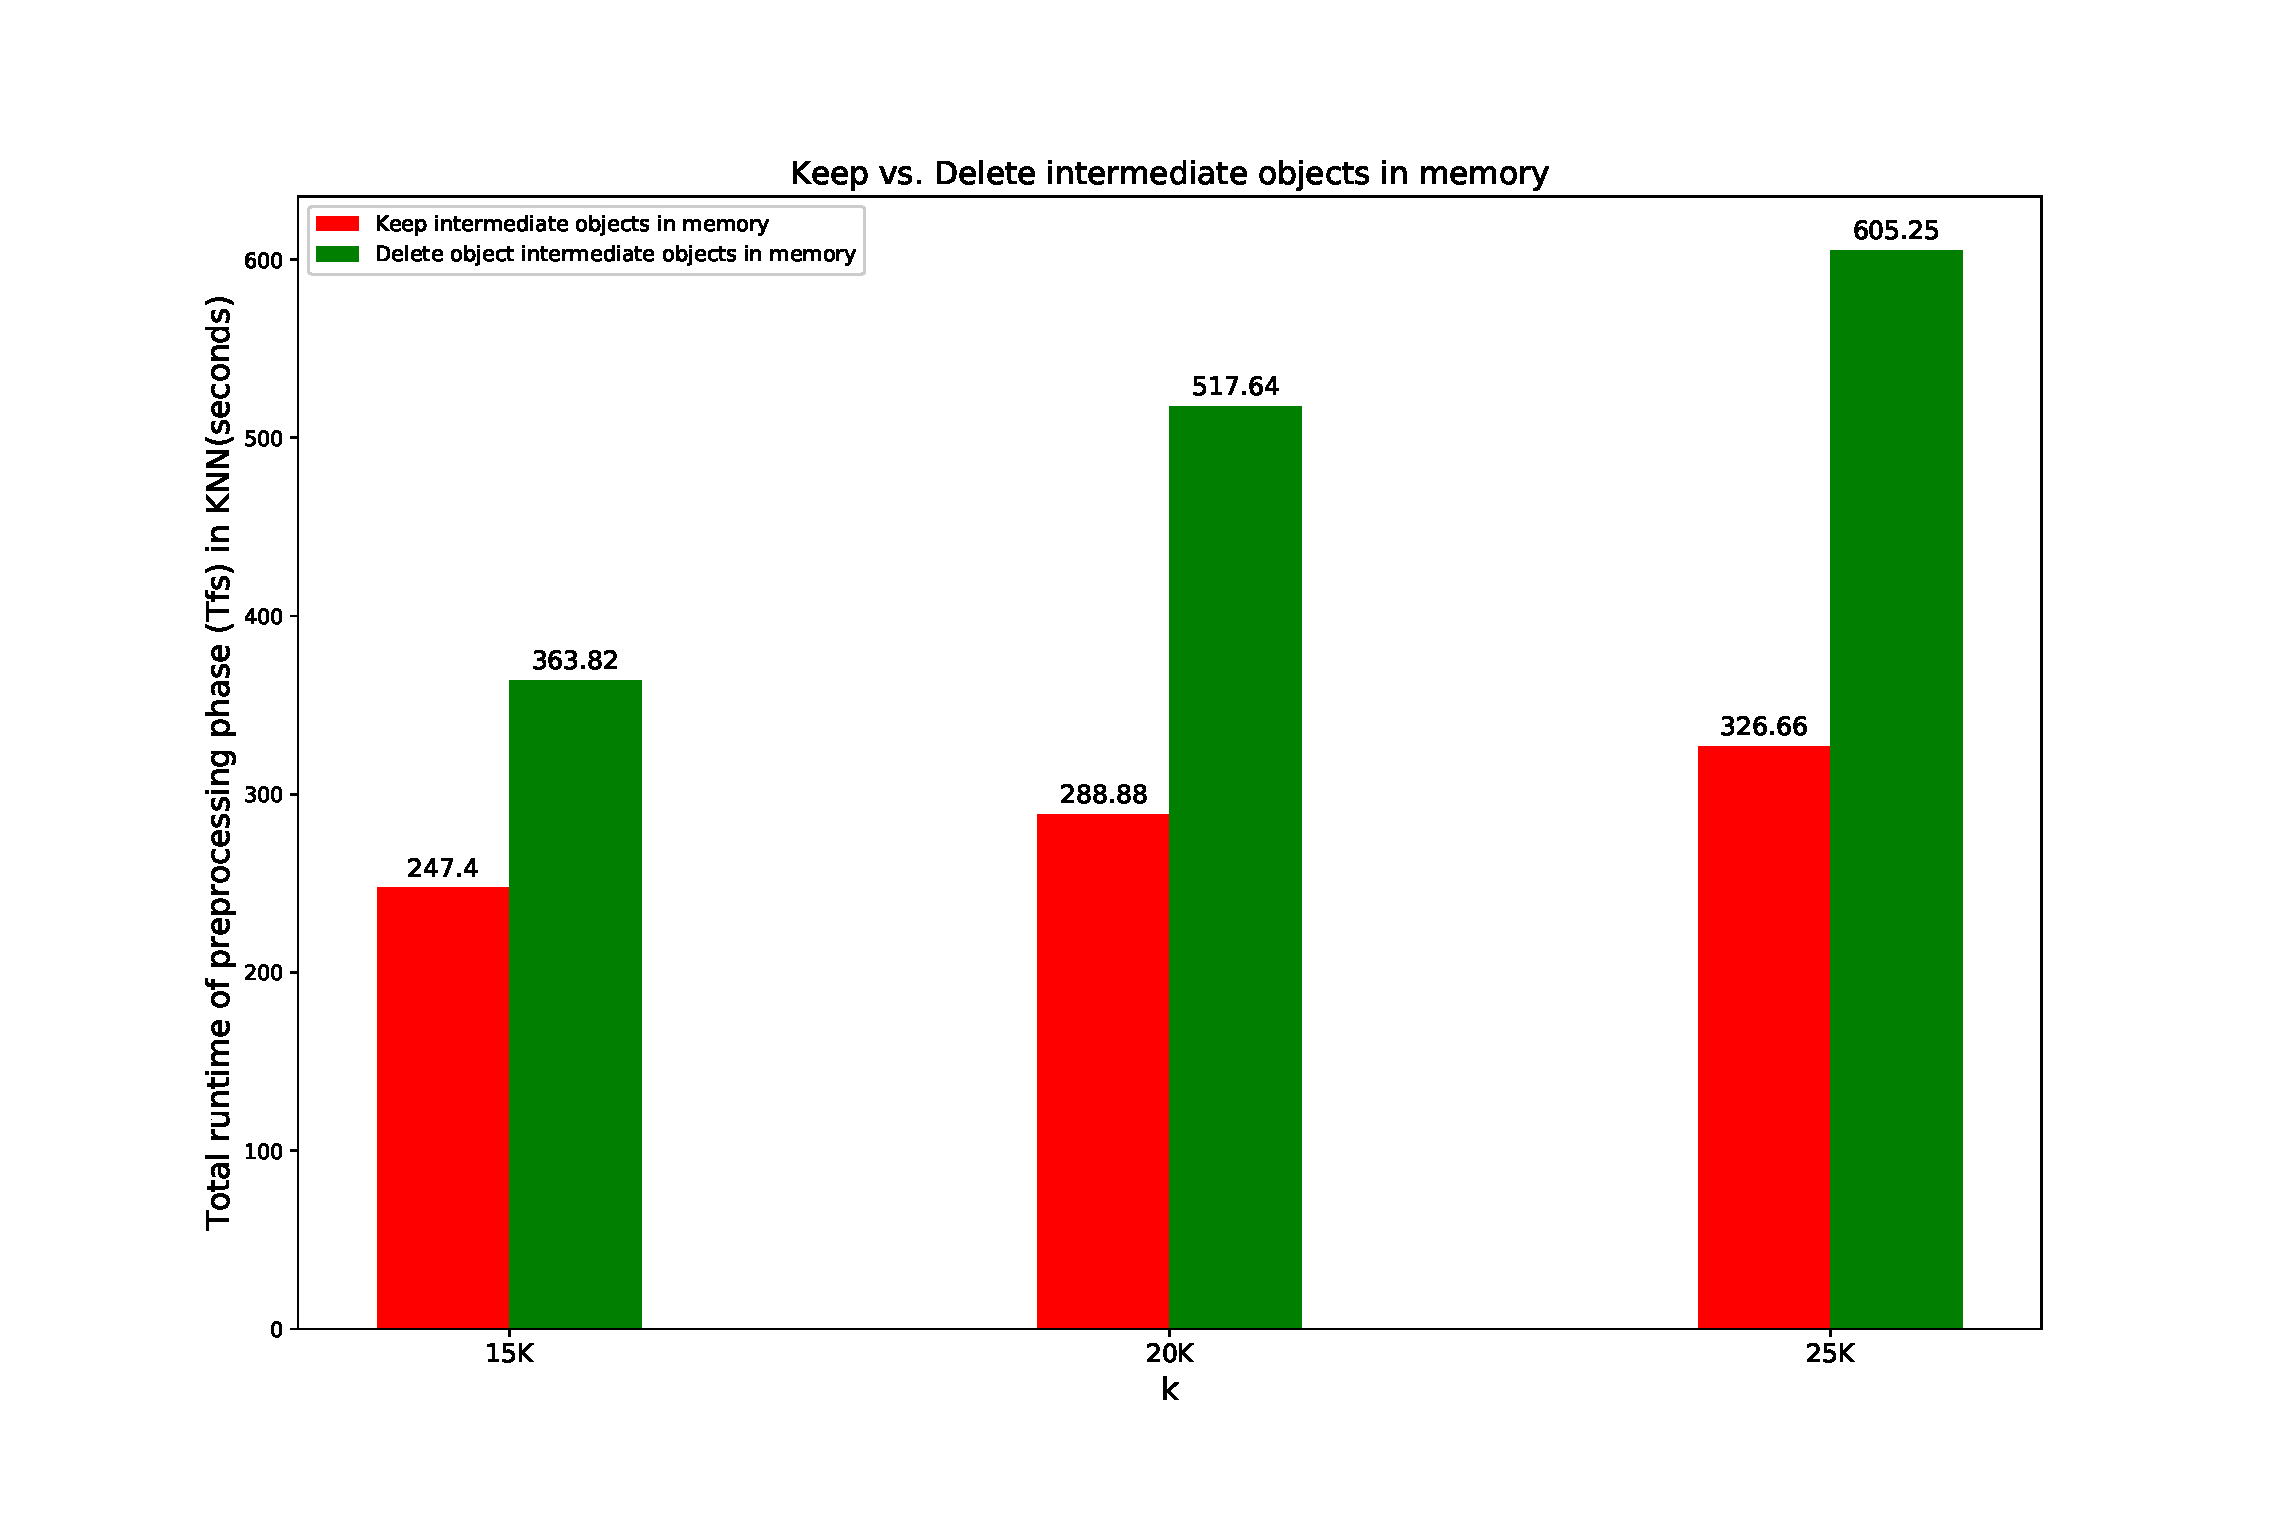
\includegraphics[width=1.1\textwidth]{images/strategy1_vs_strategy2.eps}
%                 \captionsetup{labelformat=empty}
%                 % \caption{\textbf{}}
%         \end{center}
%     \end{figure}
    
% \end{frame}

%%%%%%%%%%%%%%%%%%%%%%%%%%%%%%%%%%%%%%%%%%%%
%%%%%%%%%%%%%%%%%%%%%%%%%%%%%%%%%%%%%%%%%%%%


\begin{frame}[fragile]{Experiment 5: K-Nearest-Neighbors}
    
    \textbf{Result}
    \begin{itemize}
        \item \blueb{Arc} is \blueb{at most 38\% slower} than deep-copy.
        % \item Removing intermediate objects is \blueb{at most 85\% slower} than keeping the objects.
    \end{itemize}

    \vspace{0.5cm}

    \textbf{Discussion}
    \begin{itemize}
        \item Deep-copying String is cheaper operation than Arc: 
        \begin{itemize}
            \item reference checking
            \item atomic operation
        \end{itemize}
        % \item More frequent deallocation of intermediate objects may lead to overhead.
    \end{itemize} 
\end{frame}


%%%%%%%%%%%%%%%%%%%%%%%%%%%%%%%%%%%%%%%%%%%%
%%%%%%%%%%%%%%%%%%%%%%%%%%%%%%%%%%%%%%%%%%%%

\begin{frame}[fragile]{Findings}
    \begin{itemize}
        \item Use normal reference rather than Reference Counting whenever it is possible.
        \item Trade-off between \blueb{runtime performance} and \blueb{lifetime tracking}.
        \item \blueb{Avoid using Arc} when we can use reference.
        \item Use Arc instead of deep-copy, when \blueb{complexity of objects is large}.
        \item Use deep-copy, when \blueb{complexity of objects is small}, like String.
    \end{itemize}
\end{frame}

%%%%%%%%%%%%%%%%%%%%%%%%%%%%%%%%%%%%%%%%%%%%
%%%%%%%%%%%%%%%%%%%%%%%%%%%%%%%%%%%%%%%%%%%%

\begin{frame}[fragile]{Conclusion}
    \begin{itemize}
        \item We have seen that impact of memory memory Management is very large, 
              Specially when working on High Complex Object structures and Large Volume of Data Set. 

        \item Using a System Language like Rust is very promising to avoid using large CPU computation for memory management. 
        \item By using Rust, writing memory-safe code in multithreading is fairly easy.
         
    \end{itemize}
\end{frame}
\end{document}
